\documentclass[]{article}
\usepackage{lmodern}
\usepackage{amssymb,amsmath}
\usepackage{ifxetex,ifluatex}
\usepackage{graphicx}
\graphicspath{ {./media/} }
\usepackage{fixltx2e} % provides \textsubscript
\ifnum 0\ifxetex 1\fi\ifluatex 1\fi=0 % if pdftex
  \usepackage[T1]{fontenc}
  \usepackage[utf8]{inputenc}
\else % if luatex or xelatex
  \ifxetex
    \usepackage{mathspec}
  \else
    \usepackage{fontspec}
  \fi
  \defaultfontfeatures{Ligatures=TeX,Scale=MatchLowercase}
\fi
% use upquote if available, for straight quotes in verbatim environments
\IfFileExists{upquote.sty}{\usepackage{upquote}}{}
% use microtype if available
\IfFileExists{microtype.sty}{%
\usepackage[]{microtype}
\UseMicrotypeSet[protrusion]{basicmath} % disable protrusion for tt fonts
}{}
\PassOptionsToPackage{hyphens}{url} % url is loaded by hyperref
\usepackage[unicode=true]{hyperref}
\hypersetup{
            pdfborder={0 0 0},
            breaklinks=true}
\urlstyle{same}  % don't use monospace font for urls
\usepackage{graphicx,grffile}
\makeatletter
\def\maxwidth{\ifdim\Gin@nat@width>\linewidth\linewidth\else\Gin@nat@width\fi}
\def\maxheight{\ifdim\Gin@nat@height>\textheight\textheight\else\Gin@nat@height\fi}
\makeatother
% Scale images if necessary, so that they will not overflow the page
% margins by default, and it is still possible to overwrite the defaults
% using explicit options in \includegraphics[width, height, ...]{}
\setkeys{Gin}{width=\maxwidth,height=\maxheight,keepaspectratio}
\IfFileExists{parskip.sty}{%
\usepackage{parskip}
}{% else
\setlength{\parindent}{0pt}
\setlength{\parskip}{6pt plus 2pt minus 1pt}
}
\setlength{\emergencystretch}{3em}  % prevent overfull lines
\providecommand{\tightlist}{%
  \setlength{\itemsep}{0pt}\setlength{\parskip}{0pt}}
\setcounter{secnumdepth}{0}
% Redefines (sub)paragraphs to behave more like sections
\ifx\paragraph\undefined\else
\let\oldparagraph\paragraph
\renewcommand{\paragraph}[1]{\oldparagraph{#1}\mbox{}}
\fi
\ifx\subparagraph\undefined\else
\let\oldsubparagraph\subparagraph
\renewcommand{\subparagraph}[1]{\oldsubparagraph{#1}\mbox{}}
\fi

% set default figure placement to htbp
\makeatletter
\def\fps@figure{htbp}
\makeatother


\date{}

\begin{document}

Neuropsychiatric disease is the globally leading cause of non-fatal disease burden {[}1,
2{]}, and approximately 46\% of Americans will meet the American
Psychiatric Association's criteria for a mental disorder at some point
in their lives {[}3{]}. 
The poorly understood pathophysiology of psychiatric disorders makes them 
difficult to diagnose and has broadly precluded development of mechanism-based treatments {[}5{]}. 
In recent genetic studies, the gene \emph{CACNA1C} has consistently emerged as a
risk factor for neuropsychiatric disease, including bipolar disorder
{[}6-13{]}, schizophrenia {[}7, 14-17{]}, and major depressive disorder
{[}18, 19{]}. 
Most notably, the largest genome-wide association study to
date identified \emph{CACNA1C} as one of only two collective risk genes
among patients with bipolar disorder, schizophrenia, autism spectrum
disorders, major depressive disorder, and
attention-deficit/hyperactivity disorder {[}15, 20{]}. 
Nearly a decade after first being implicated in psychiatric disorders, the role of
\emph{CACNA1C} in psychopathology remains unclear.

\begin{figure}[h]
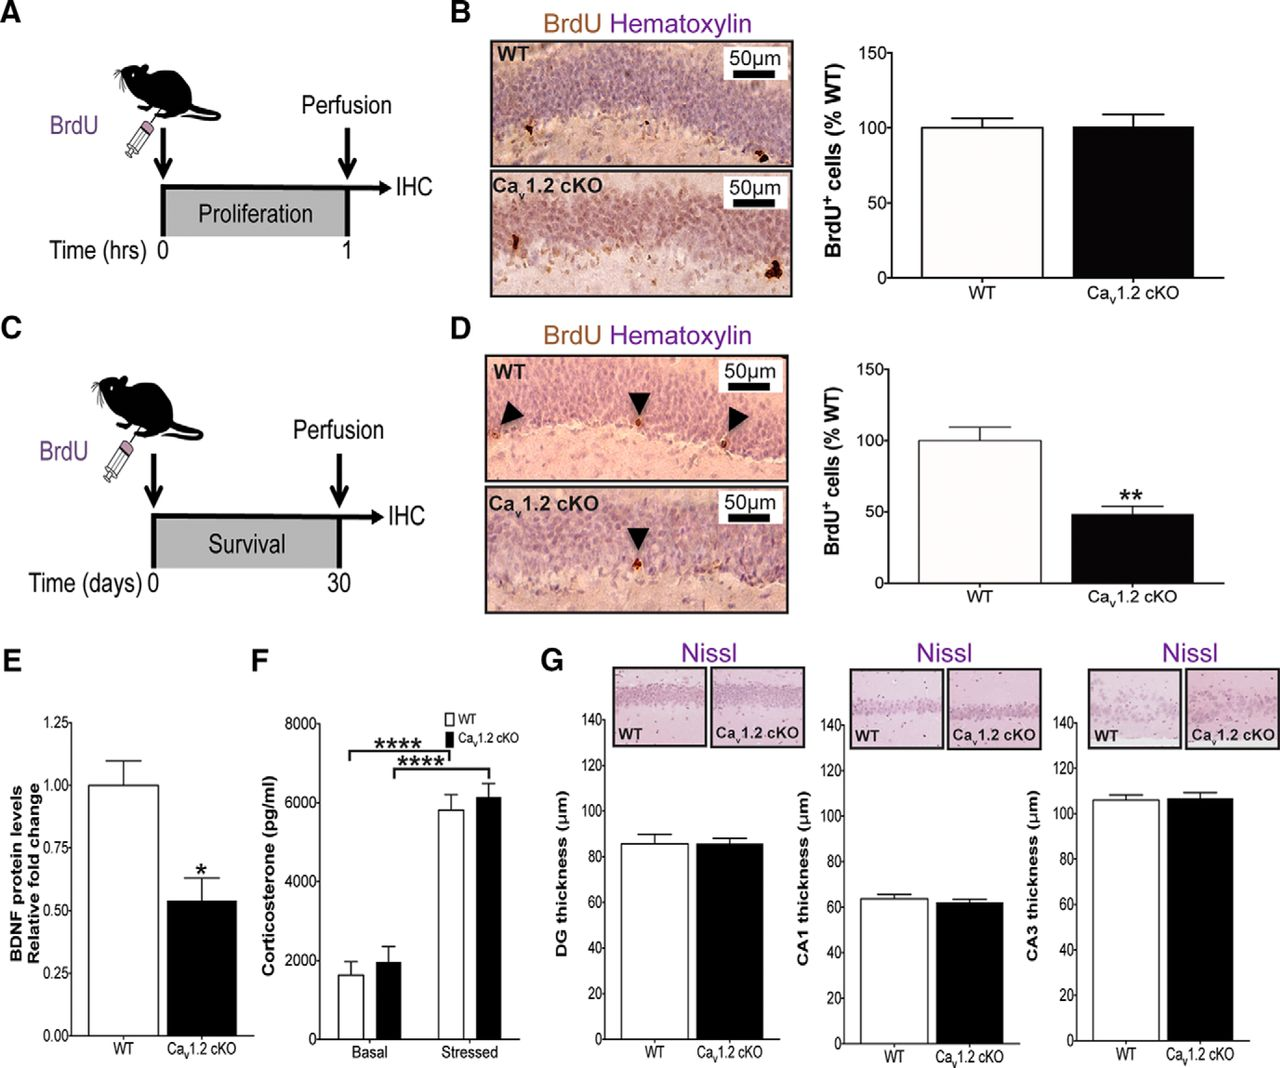
\includegraphics{image.jpg}
	\caption{Figure 1: Forebrain-specific knockout of Cav1.2 reduces the survival of newborn neurons.
		Mice were given a single injection of bromodeoxyuridine (BrdU) and sacrificed 30 days later. Brains were serially sectioned and the number of BrdU-positive (BrdU+) neurons were quantified between genotypes. **p<0.01 [4]}
\end{figure}

\emph{CACNA1C} encodes Ca\textsubscript{v}1.2, which comprises 85\% of
voltage-gated L-type calcium channel (LTCC) alpha subunits in the
mammalian brain and confers much of the whole channel's functional
properties, including drug sensitivity, selectivity, and composition of
both the pore-forming unit and voltage-sensing domain {[}21-23{]}.
Ca\textsubscript{v}1.2 has a well-established role in coupling
postsynaptic membrane depolarization with expression of genes involved
in long term potentiation and concomitant memory formation {[}24-30{]}.
Previously, our research group assessed the consequences of
forebrain-specific elimination of \emph{Cacna1c} on mouse postnatal
hippocampal neurogenesis. 
Using this model, we identified a two-fold increase in young hippocampal 
neuron death, providing evidence for Ca\textsubscript{v}1.2 as a key regulator
 of neuronal survival in postnatal hippocampal neurogenesis (Figure 1) {[}4{]}.

Cell death is a prominent feature of many forms of neuropsychiatric
illness {[}31{]} and can result from an array of mechanisms, including
necrosis, autophagy, and apoptosis {[}32{]}. 
Importantly, loss of mitochondrial calcium homeostasis predisposes neurons to activation of
cell death programs, placing mitochondria as pivotal regulators in
neuronal life and death {[}33-39{]}. 
Energy-demanding tissues in the nervous system require 
tightly regulated mitochondrial calcium (Ca\textsuperscript{2+}) 
for efficient production of adenosine triphosphate (ATP) {[}35, 40, 41{]}.

Ca\textsubscript{v}1.2 activity itself increases mitochondrial
metabolism and reactive oxygen species (ROS) levels, likely due to
allosteric activation of Ca\textsuperscript{2+}-sensitive tri-carboxylic
acid (TCA) cycle dehydrogenases and ATP synthase {[}42{]}. 
Persistently elevated Ca\textsuperscript{2+} levels push ROS production beyond
tolerable signaling levels and lower the threshold for opening of the
mitochondria permeability transition pore (PTP), priming mitochondria
cytochrome C release and apoptosis {[}33-36{]}. 
In renal tubular cells, blockade of LTCCs reduces both mitochondrial Ca\textsuperscript{2+}
accumulation and mitochondria-mediated apoptosis {[}43-46{]}. 
In addition, patients with bipolar disorder, schizophrenia, and major
depression show deficits in neuronal oxidative phosphorylation {[}47, 48{]}. 
The links between Ca\textsubscript{v}1.2 and mitochondria in
calcium flux and cell death raise the possibility that altered
Ca\textsubscript{v}1.2 signaling in psychiatric disorders could disrupt
intracellular calcium (Ca\textsuperscript{2+}) handling in mitochondria
and prime neurons for apoptosis.

1. Murray, C.J.L., et al., \emph{Disability-adjusted life years (DALYs)
for 291 diseases and injuries in 21 regions, 1990--2010: a systematic
analysis for the Global Burden of Disease Study 2010.} The Lancet, 2012.
\textbf{380}(9859): p. 2197-2223.

2. Whiteford, H.A., et al., \emph{Global burden of disease attributable
to mental and substance use disorders: findings from the Global Burden
of Disease Study 2010.} The Lancet, 2013. \textbf{382}(9904): p.
1575-1586.

3. Kessler, R.C., et al., \emph{LIfetime prevalence and age-of-onset
distributions of dsm-iv disorders in the national comorbidity survey
replication.} Archives of General Psychiatry, 2005. \textbf{62}(6): p.
593-602.

4. Lee, A.S., et al., \emph{The Neuropsychiatric Disease-Associated Gene
cacna1c Mediates Survival of Young Hippocampal Neurons.} eneuro, 2016.
\textbf{3}(2).

5. Bhat, S., et al., \emph{CACNA1C (Cav1.2) in the pathophysiology of
psychiatric disease.} Prog Neurobiol, 2012. \textbf{99}(1): p. 1-14.

6. Ferreira, M.A., et al., \emph{Collaborative genome-wide association
analysis supports a role for ANK3 and CACNA1C in bipolar disorder.} Nat
Genet, 2008. \textbf{40}(9): p. 1056-8.

7. Moskvina, V., et al., \emph{Gene-wide analyses of genome-wide
association data sets: evidence for multiple common risk alleles for
schizophrenia and bipolar disorder and for overlap in genetic risk.} Mol
Psychiatry, 2009. \textbf{14}(3): p. 252-60.

8. Baum, A.E., et al., \emph{A genome-wide association study implicates
diacylglycerol kinase eta (DGKH) and several other genes in the etiology
of bipolar disorder.} Mol Psychiatry, 2007. \textbf{13}(2): p. 197-207.

9. Sklar, P., et al., \emph{Large-scale genome-wide association analysis
of bipolar disorder identifies a new susceptibility locus near ODZ4.}
Nature genetics, 2011. \textbf{43}(10): p. 977.

10. Sklar, P., et al., \emph{Whole-genome association study of bipolar
disorder.} Mol Psychiatry, 2008. \textbf{13}(6): p. 558-69.

11. Lee, M.T.M., et al., \emph{Genome-wide association study of bipolar
I disorder in the Han Chinese population.} Molecular psychiatry, 2011.
\textbf{16}(5): p. 548-556.

12. Nurnberger, J.I., et al., \emph{Identification of pathways for
bipolar disorder: a meta-analysis.} JAMA psychiatry, 2014.
\textbf{71}(6): p. 657-664.

13. Ament, S.A., et al., \emph{Rare variants in neuronal excitability
genes influence risk for bipolar disorder.} Proceedings of the National
Academy of Sciences, 2015. \textbf{112}(11): p. 3576-3581.

14. Nyegaard, M., et al., \emph{CACNA1C (rs1006737) is associated with
schizophrenia.} Mol Psychiatry, 2010. \textbf{15}(2): p. 119-21.

15. Cross-Disorder Group of the Psychiatric Genomics Consortium, et al.,
\emph{Genetic relationship between five psychiatric disorders estimated
from genome-wide SNPs.} Nat Genet, 2013. \textbf{45}(9): p. 984-94.

16. Ripke, S., et al., \emph{Genome-wide association analysis identifies
13 new risk loci for schizophrenia.} Nature genetics, 2013.
\textbf{45}(10): p. 1150-1159.

17. Green, E.K., et al., \emph{Replication of bipolar disorder
susceptibility alleles and identification of two novel genome-wide
significant associations in a new bipolar disorder case--control
sample.} Molecular psychiatry, 2013. \textbf{18}(12): p. 1302-1307.

18. Green, E.K., et al., \emph{The bipolar disorder risk allele at
CACNA1C also confers risk of recurrent major depression and of
schizophrenia.} Mol Psychiatry, 2010. \textbf{15}(10): p. 1016-22.

19. Casamassima, F., et al., \emph{Phenotypic effects of a bipolar
liability gene among individuals with major depressive disorder.}
American Journal of Medical Genetics Part B: Neuropsychiatric Genetics,
2010. \textbf{153}(1): p. 303-309.

20. The Wellcome Trust Case Control Consortium, \emph{Genome-wide
association study of 14,000 cases of seven common diseases and 3,000
shared controls.} Nature, 2007. \textbf{447}(7145): p. 661-678.

21. Seisenberger, C., et al., \emph{Functional Embryonic Cardiomyocytes
after Disruption of the L-type $\alpha$1C (Ca v 1.2) Calcium Channel Gene in
the Mouse.} Journal of Biological Chemistry, 2000. \textbf{275}(50): p.
39193-39199.

22. Zamponi, G.W., \emph{Targeting voltage-gated calcium channels in
neurological and psychiatric diseases.} Nat Rev Drug Discov, 2016.
\textbf{15}(1): p. 19-34.

23. Sinnegger-Brauns, M.J., et al., \emph{Expression and
1,4-Dihydropyridine-Binding Properties of Brain L-Type Calcium Channel
Isoforms.} Molecular Pharmacology, 2009. \textbf{75}(2): p. 407-414.

24. Gerald J. Obermair, Z.S., Emmanuel Bourinet, Bernhard E. Flucher,
\emph{Differential targeting of the L-type Ca2+ channel a1c (Cav1.2) to
synaptic and extrasynaptic compartments in hippocampal neurons.}
European Journal of Neuroscience, 2004. \textbf{19}: p. 2109-2122.

25. Moosmang, S., et al., \emph{Role of hippocampal Cav1.2 Ca2+ channels
in NMDA receptor-independent synaptic plasticity and spatial memory.} J
Neurosci, 2005. \textbf{25}(43): p. 9883-92.

26. Bading, H., D. Ginty, and M. Greenberg, \emph{Regulation of gene
expression in hippocampal neurons by distinct calcium signaling
pathways.} Science, 1993. \textbf{260}(5105): p. 181-186.

27. Anirvan Ghosh, J.C., Michael E. Greenberg, \emph{Requirement for
BDNF in Activity-Dependent Survival of Cortical Neurons.} Science, 1994.
\textbf{263}: p. 1618-1623.

28. Deisseroth, K., et al., \emph{Signaling from synapse to nucleus: the
logic behind the mechanisms.} Current Opinion in Neurobiology, 2003.
\textbf{13}(3): p. 354-365.

29. Zakharenko, S.S., et al., \emph{Presynaptic BDNF Required for a
Presynaptic but Not Postsynaptic Component of LTP at Hippocampal CA1-CA3
Synapses.} Neuron, 2003. \textbf{39}(6): p. 975-990.

30. Zhang, Q., et al., \emph{The Effects of CACNA1C Gene Polymorphism on
Spatial Working Memory in Both Healthy Controls and Patients with
Schizophrenia or Bipolar Disorder.} Neuropsychopharmacology, 2012.
\textbf{37}(3): p. 677-684.

31. Dodd, S., et al., \emph{Putative neuroprotective agents in
neuropsychiatric disorders.} Progress in Neuro-Psychopharmacology and
Biological Psychiatry, 2013. \textbf{42}: p. 135-145.

32. Fink, S.L. and B.T. Cookson, \emph{Apoptosis, pyroptosis, and
necrosis: mechanistic description of dead and dying eukaryotic cells.}
Infect Immun, 2005. \textbf{73}(4): p. 1907-16.

33. Das, A.M. and D.A. Harris, \emph{Control of mitochondrial ATP
synthase in heart cells: inactive to active transitions caused by
beating or positive inotropic agents.} Cardiovascular Research, 1990.
\textbf{24}(5): p. 411-417.

34. Hajnoczky, G., et al., \emph{Mitochondrial calcium signalling and
cell death: approaches for assessing the role of mitochondrial Ca2+
uptake in apoptosis.} Cell Calcium, 2006. \textbf{40}(5-6): p. 553-60.

35. Brookes, P.S., et al., \emph{Calcium, ATP, and ROS: a mitochondrial
love-hate triangle.} American Journal of Physiology - Cell Physiology,
2004. \textbf{287}(4): p. C817-C833.

36. Wang, W., G. Karamanlidis, and R. Tian, \emph{Novel targets for
mitochondrial medicine.} Science Translational Medicine, 2016.
\textbf{8}(326): p. 326rv3-326rv3.

37. Liu, X., et al., \emph{Induction of apoptotic program in cell-free
extracts: Requirement for dATP and cytochrome c.} Cell, 1996.
\textbf{86}(1): p. 147-157.

38. Yang, J., et al., \emph{Prevention of apoptosis by Bcl-2: Release of
cytochrome c from mitochondria blocked.} Science, 1997.
\textbf{275}(5303): p. 1129-1132.

39. Nicholls, D.G., \emph{Mitochondrial calcium function and dysfunction
in the central nervous system.} Biochimica et biophysica acta, 2009.
\textbf{1787}(11): p. 1416-1424.

40. Viola, H.M. and L.C. Hool, \emph{Cross-talk between L-type Ca2+
channels and mitochondria.} Clinical and Experimental Pharmacology and
Physiology, 2010. \textbf{37}(2): p. 229-235.

41. Fattal, O., et al., \emph{Review of the Literature on Major Mental
Disorders in Adult Patients With Mitochondrial Diseases.}
Psychosomatics, 2006. \textbf{47}(1): p. 1-7.

42. Viola, H.M., P.G. Arthur, and L.C. Hool, \emph{Evidence for
regulation of mitochondrial function by the L-type Ca2+ channel in
ventricular myocytes.} Journal of Molecular and Cellular Cardiology,
2009. \textbf{46}(6): p. 1016-1026.

43. Tanaka, T., et al., \emph{Blockade of Calcium Influx through L-Type
Calcium Channels Attenuates Mitochondrial Injury and Apoptosis in
Hypoxic Renal Tubular Cells.} Journal of the American Society of
Nephrology, 2004. \textbf{15}(9): p. 2320-2333.

44. Singh, A., et al., \emph{Nimodipine, an L-type calcium channel
blocker attenuates mitochondrial dysfunctions to protect against
1-methyl-4-phenyl-1,2,3,6-tetrahydropyridine-induced Parkinsonism in
mice.} Neurochemistry International, 2016. \textbf{99}: p. 221-232.

45. Sun, M., et al., \emph{CNTF-ACM promotes mitochondrial respiration
and oxidative stress in cortical neurons through upregulating L-type
calcium channel activity.} Molecular and Cellular Biochemistry, 2016.
\textbf{420}(1): p. 195-206.

46. Saberzadeh, J., M. Omrani, and M.A. Takhshid, \emph{Protective
effects of nimodipine and lithium against aluminum-induced cell death
and oxidative stress in PC12 cells.} Iran J Basic Med Sci, 2016.
\textbf{19}(2008-3866 (Print)): p. 1251-1257.

47. Rezin, G.T., et al., \emph{Mitochondrial Dysfunction and Psychiatric
Disorders.} Neurochemical Research, 2008. \textbf{34}(6): p. 1021-1029.

48. Kato, T. and N. Kato, \emph{Mitochondrial dysfunction in bipolar
disorder.} Bipolar Disorders, 2000. \textbf{2}(3): p. 180-190.

\end{document}
